\chapter{Introduction}
\label{chap:introduction}

The longer and more complex a source code is, the more difficult it is to verify its correctness.
There are different approaches to show the correctness of a program.
One of them is formal verification.
In contrast to testing, where only predefined inputs are tested, with formal verification all possible inputs are covered.
The correctness of a program is analyzed relative to its formal specification.
Formal specification is a mathematical description of a software behavior that can be used by the verification tool to verify the code.
We will see an example of a formal specification shortly.

In this work we use the verification framework Stainless to verify parts of the code of Bitcoin-S, a Scala implementation of the Bitcoin protocol.
In the following we look at the main aspects of formal verification with Stainless and properties of Bitcoin-S we want to verify.


\section{Formal Verification with Stainless}
\label{sec:stainless}

Stainless is developed by "Lab for Automated Reasoning and Analysis" (LARA) at EPFL's School of Computer and Communication Sciences.
Using this framework we can verify the correctness of Scala programs.
The following overview of the framework is taken from the section \href{https://epfl-lara.github.io/stainless/intro.html}{Introduction} of the Stainless documentation \cite{Stainless:documentation}.

Stainless statically verifies that a program satisfies a given specification and that a program will not crash at runtime.
The framework covers all possible inputs and finds a counter examples for possible failures in a program which violate the given specification.

The main functions used to write a specification are \textit{require} and \textit{ensuring}.

With \textit{require} we define a precondition of a function, which we want to verify.
\textit{require} is placed at the beginning of the function body.
\textit{require} specifies, if the parameter of the function holds against a certain condition.

With \textit{ensuring}, we define the postcondition of a function.
\textit{ensuring} is placed at the end of the function after the body.
\textit{ensuring} specifies, if the return value or the result of the function satisfies a certain condition.

On invoking Stainless, it tries to prove that the postcondition always holds, assuming the given precondition does hold.

The following example demonstrates a simple formal specification for the function calculating a factorial.
This is a modified example from the section \href{https://epfl-lara.github.io/stainless/intro.html}{Introduction} of the Stainless documentation \cite{Stainless:documentation}, so Stainless reports an error verifying it.
\begin{lstlisting}[language=Scala]
  def factorial(n: Int): Int = {
      require(n >= 0)
      if (n == 0) {
        1
      } else {
        n * factorial(n - 1)
      }
  } ensuring(res => res >= 0)
\end{lstlisting}

It recursively calculates the factorial of an integer number.
The input of the function is constrained with \textit{require} to a non-negative value.
The result should also be non-negative.
Thus, Stainless will verify whether the result of the factorial calculation is non-negative for all non-negative inputs.

Stainless can produce 3 outcomes of postcondition verification: \textit{valid}, \textit{invalid} and \textit{unknown}.
If the postcondition is \textit{valid} Stainless could prove that for any inputs constrained in the precondition, the postcondition always holds.
Reporting the postcondition as \textit{invalid} the framework could find at least one counterexample which satisfies the precondition but violates the postcondition.
If Stainless is unable to prove the postcondition or find a counterexample it reports the outcome \textit{unknown}.
In this case a timeout or an internal error occurred.
Furthermore, Stainless checks for calls in the code to the function with invalid arguments violating the precondition.
For example if we invoke factorial with a negative number it reports \textit{invalid}.

Let's return to our incorrect example with factorial.
Stainless reports the following result for the factorial verification from our example:
\begin{figure}[H]
	\centering
		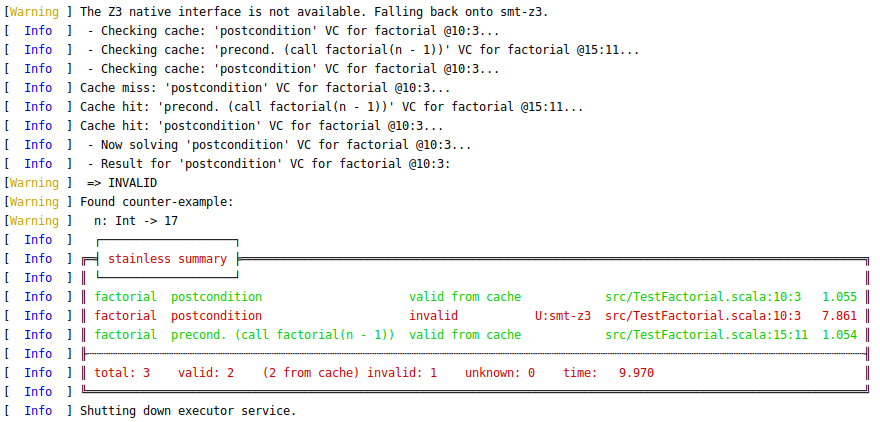
\includegraphics[scale=0.5]{images/output1.png}
	\caption{Output of Stainless verification for calculating factorial of Int number}
	\label{fig:output1}
\end{figure}

Stainless disproves the postcondition and gives the number 17 as a counterexample.
Due to an overflow in the 32 bit Int the result becomes a negative value.
The program would work correct by changing the type from Int to BigInt.

Stainless supports only a subset of Scala.
They call this Pure Scala.
You can find the specification of Pure Scala on the Stainless documentation website \cite{Stainless:documentation} in the section \href{https://epfl-lara.github.io/stainless/purescala.html}{Pure Scala}.

In addition, Stainless has its own library with annotations, reimplementation of some core data types, collections and input-output functions and more.
Some of them are described on the website in the section \href{https://epfl-lara.github.io/stainless/library.html}{Stainless Library}.
There are more details about the library in the source code of Stainless on GitHub \cite{Stainless:github} in the folder \href{https://github.com/epfl-lara/stainless/tree/master/frontends/library/stainless}{\textit{frontends/library/stainless}}.

Stainless verifies Scala programs using SMT (satisfiability modulo theories) solvers. 


\section{The Properties to Verify}

Bitcoin-S is a large project found on GitHub implementing many functionalities.
In this work we look at two of them, namely the \nameref{property_1} and the \nameref{property_2} described shortly.
Thus, we go through the relevant code parts to verify those properties, look at some challenges with Stainless and see why we should write software with verification in mind.
In order to be able to verify Bitcoin-S, we have to rewrite parts of it in the subset of Scala supported by Stainless.


\subsection{No-Inflation Property}
\label{property_1}

The decision to verify this property was inspired by the bug found in Bitcoin Core in September 2018  \cite{cve201817144} which allowed to spend the same unspent transaction output (UTXO) in a transaction multiple times.
Hence, new coins could be created out of the air.
Thus, we try to verify the property, that a non-coinbase transaction cannot generate new coins.
Let's name it the \nameref{property_1}.

As we can see later in chapter \ref{chap:verify_check}, we must rewrite a huge part of the code implementing this property.
This reimplementation into Pure Scala needs a lot of time.
So, we adjust the plan and verify another functionality of Bitcoin-S.
Nevertheless, during the analysis of the \nameref{property_1} we look at a bug in Bitcoin-S found during this work and see the code changes for the bugfix in section \ref{sec:bugfix}. 


\subsection{Addition-with-Zero Property}
\label{property_2}

In Bitcoin-S there is a class \texttt{Satoshis} representing an amount of bitcoins.
We look at the verification of the addition of Satoshis with zero Satoshis.
This operation should result in the same amount of Satoshis.
Let's call it the \nameref{property_2}.

Using Stainless, we see the successful verification of this property.
But the process of the verification with the tool requires many changes in the code, so that Stainless can accept it.
We look at all needed modifications in chapter \ref{chap:verify_add}.
